\section{实验一：相同电流维数，比较完整材料步}
实验中的每个模型最终保留相同的$k=4,8,16$列复电流，所有照明共用这个空间。完整正问题、材料注入、残差、prior和LM阻尼一致；唯一改变的是电流空间里保留哪些方向。较大的anchor和dictionary只是取得候选的辅助信息，不算进最终电流秩，却必须计入费用。

使用三维矢量Maxwell DDA，计算域边长1.5，波数$k_0=2$；反演网格$12^3$、生成数据的网格$14^3$。六次平面波照明、64个双极化接收器。两张网格都来自同一DDA实现族，因此较细网格可以减轻正反问题使用完全相同离散模型造成的过于理想评估（inverse crime），但不等同于另一个独立全波求解器。材料方向使用体积加权正交Gaussian或voxel展开，极化率导数保留。

对每个对象，取初始化、保存迭代索引3及最后保存的状态，再比较三个电流预算。我们先在对象内部对所有绝对GN gap求和，然后计算
\[
\rho_{\rm obj}=\frac{\sum R_{\rm exchange}}{\sum R_{\rm receiver}}.
\]
小于1说明这种空间选择让该对象的材料步更接近完整GN步。它不意味着材料真值误差也减少相同比例。状态与预算是同一对象上的相关观测；对象才是统计汇总单位。

\subsection{原四对象：有明确收益，不能代替外部检验}
四对象分别为平滑Gaussian、近接触Gaussian、分层voxel、非对称voxel。36个单元中35个改善、1个相同，四个对象风险比分别为0.1904、0.6538、0.2776、0.4181，中位0.3478，即完整GN gap中位下降65.2\%。这些对象参与过方法形成，因此单靠它们不能证明推广效果。更换在线阈值后，36个单元的真实物理回放保持75次接受、全部终态空间和材料步逐位一致，说明部署定义修正没有改变这一结果。

\subsection{额外对象：规则锁定以后，十个完整对象都改善}
所有十一项兼容资产在看到交换结果前进入预先锁定的资产清单（manifest）。十个对象完整提供九个单元，均改善；中位风险比0.4928，下降50.7\%。四分位区间为[0.3314,0.5588]，按对象重采样（object bootstrap）得到的中位数95\%区间为[0.3133,0.5647]。另外一个非对称voxel对象完成六个早/中期单元，比值0.4925；晚期第一个预算的receiver端点没有通过预设法方程残差（normal-equation residual）检查，其余两个预算未运行。故覆盖是96/99，不能写成99/99成功。

\begin{figure}[htbp]\centering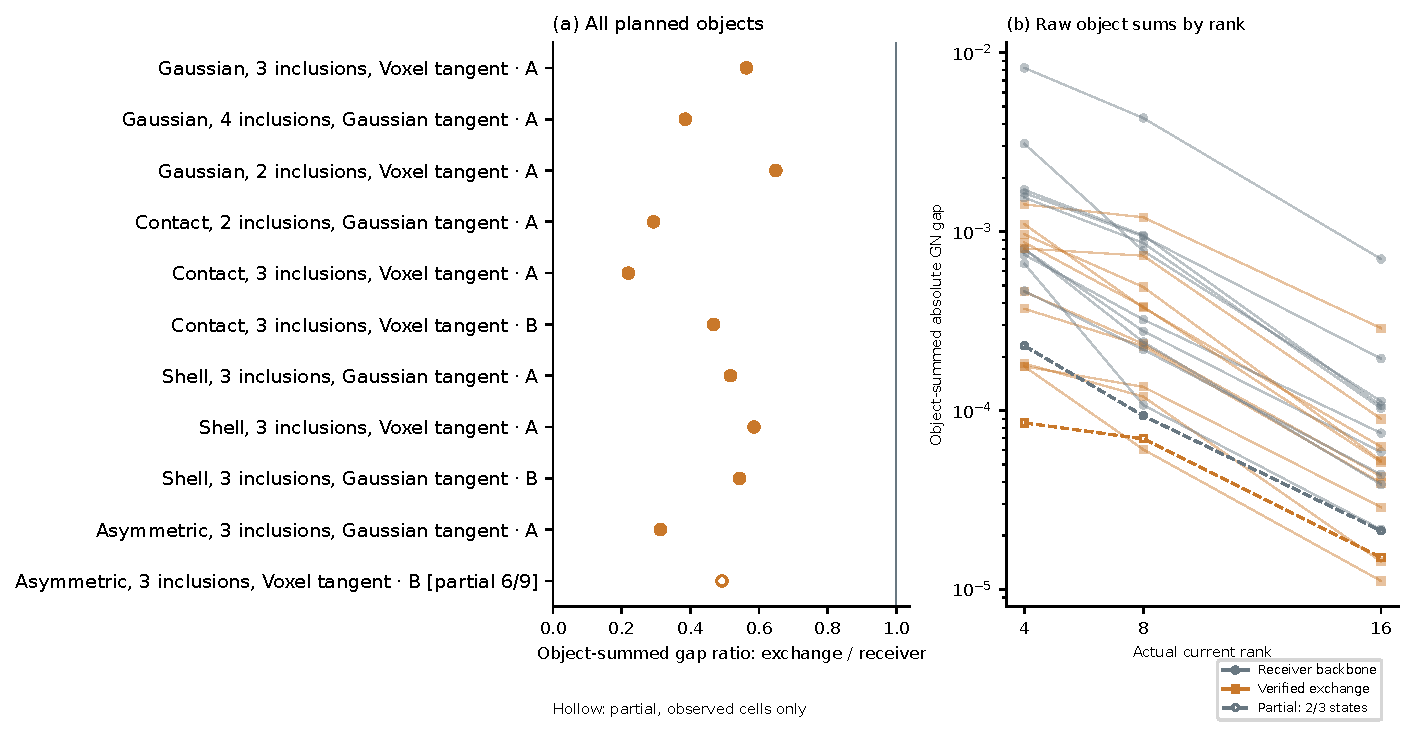
\includegraphics[width=.98\linewidth]{figures/closure_validation_v2/Figure1_primary_overview.pdf}
\caption{怎样读图：左图每个点对应一个对象的gap总和比值，1表示没有改善；空心点只有六个单元。右图把不同电流秩下的绝对gap同时画出，灰色为receiver，橙色为exchange；虚线表示该对象只有两个状态。较高电流秩通常使两种gap都变小，但仍需逐对象比较。}
\end{figure}

96个有效单元中95个改善、1个相同。receiver绝对gap范围为$2.74\times10^{-7}$至$3.09\times10^{-3}$，exchange为$8.73\times10^{-8}$至$8.36\times10^{-4}$。最小分母仍是对应evaluation floor的$6.31\times10^9$倍；最大完整参考真相对法方程残差为$9.55\times10^{-12}$。这说明下降不是参考底噪放大的假象。

这些资产曾用于宽域电流选择研究。没有找到它们用于历史交换的离线完整收益参考（exchange teacher）或试验网络（network pilot）的记录，但也不能保证历史结果完全没有影响过方法判断。因此准确说法是“冻结规则在额外、曾研究过的Maxwell对象上得到验证”，而不是“全新独立盲测”。Bootstrap描述固定对象集合中的变化范围，不能自动推广到所有物体分布。

\section{实验二：噪声改变材料要求，重新评价而不沿用干净参考}
加噪声不是把原来的表再抖动一下：$r$改变以后，完整GN最优步本来就不同，所以每份noisy residual必须重新有自己的离线reference。我们固定四个对象的中期材料和物理算子，加入精确相对范数1\%与3\%的复高斯噪声，每级三份独立噪声样本（realization），保持相同归一化尺度和冻结规则。

72/72单元通过来源和质量审计；71个改善、1个no-op。四对象在1\%噪声下的汇总比值为0.3255、0.0996、0.3358、0.3687，中位0.3307；3\%下为0.4384、0.1873、0.3667、0.5330，中位0.4026。局部材料步收益在这个有限测试中仍然存在。

\begin{figure}[htbp]\centering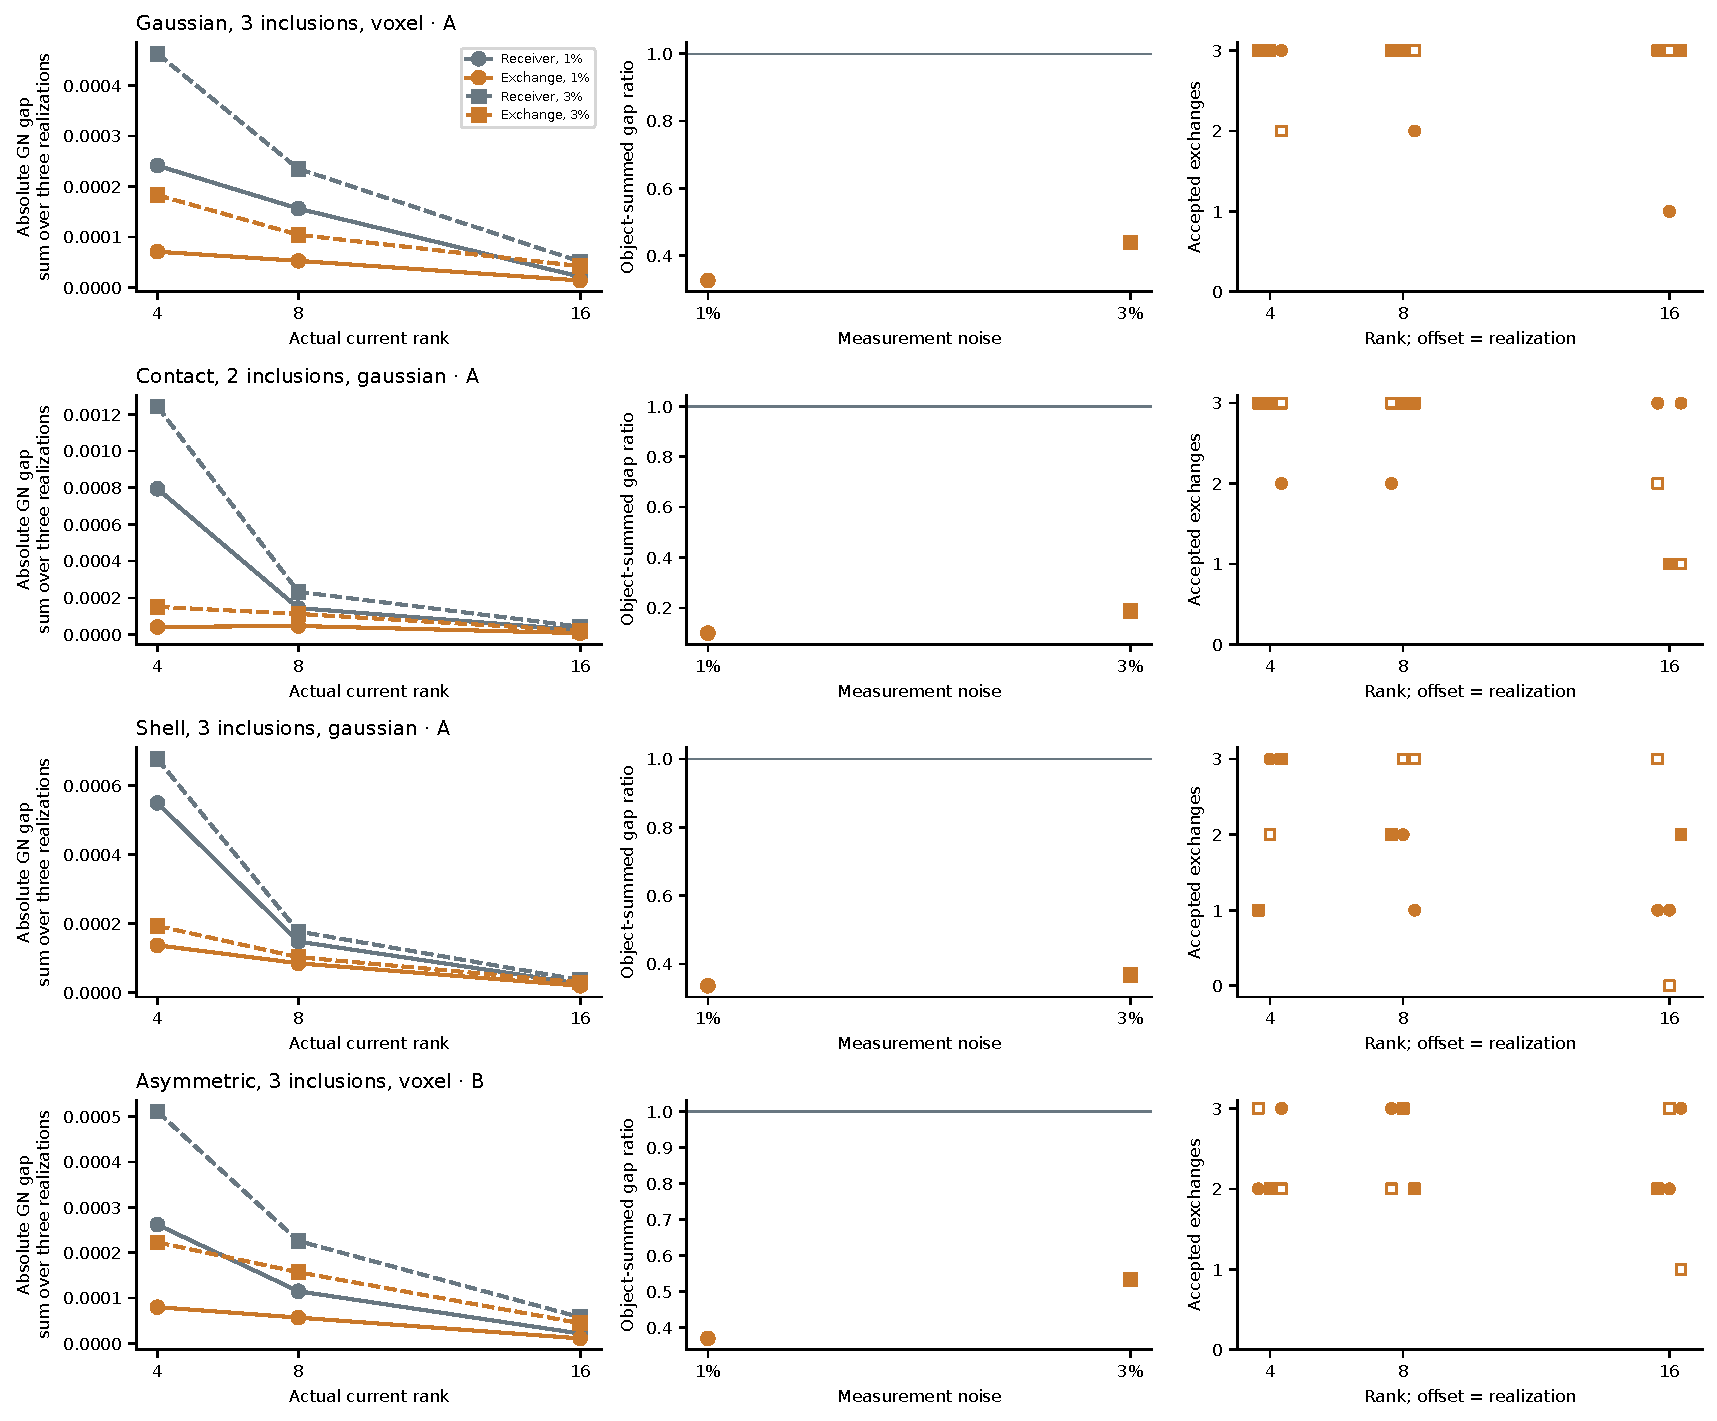
\includegraphics[width=.98\linewidth]{figures/closure_validation_v1/Figure2_noise_objects.pdf}
\caption{每行一个预选对象：左列给出三份realization的绝对gap之和，中列是对象风险比，右列是每份噪声接受了多少交换。此图没有把realization作为新的独立对象。噪声增大时某些对象收益减弱，但全部对象汇总比值仍小于1。}
\end{figure}

模式本身没有保持不变。根据保存的物理基底计算主角度（principal angles，用于衡量两个物理子空间的偏离），70/72终态相对干净情况至少有一个方向偏转10°以上，65/72达到80°以上。这是部分方向的变化，不是整个空间都被替换。材料用途依赖残差，变化可以是合理响应；所以这里报告的是收益稳定出现，而不是宣称方向选择具有不变性。

408个finalist中98个被数值复核拒绝，共接受172次交换。Jd使用2448个电流方程右端（current right-hand sides, RHS），算入Jx初始化后为2880。完整噪声作业占用895.250s；scoring、传输和Jd等嵌套阶段已包括其中。这个结果只涵盖四对象、中期、两级噪声与三份realization，不足以宣称普遍统计鲁棒性。

\section{候选覆盖：评分准确仍可能错过好方向}
假设我们知道怎样给替换打分，但只看12个移入方向。如果最有用的方向在第13个之外，再好的打分公式也选不到它。为检验这一点，离线teacher枚举固定154方向字典中的整个初次交换邻域（initial exchange neighborhood）：保留$k$列时，共有$k(154-k)$个一换一组合。无效端点照样记录；完整收益标注在部署完成之后获取，不进入selector。

令每个单元的全字典最大正收益为$Q_*^+=\max(0,\max Q)$。对象内先对这些机会求和，再用anchor选中且通过方向复核的收益之和除以它，得到排序机会捕获率（ranking opportunity capture）。十个完整额外对象为97.30--99.99\%，中位99.54\%。同样计算12候选池内最好收益可覆盖的机会，得到候选覆盖率（candidate opportunity coverage）：49.12--95.31\%，中位72.95\%。零机会不提供权重；未完成对象只有六单元的观察值，不能填成九单元总体。

\begin{figure}[htbp]\centering
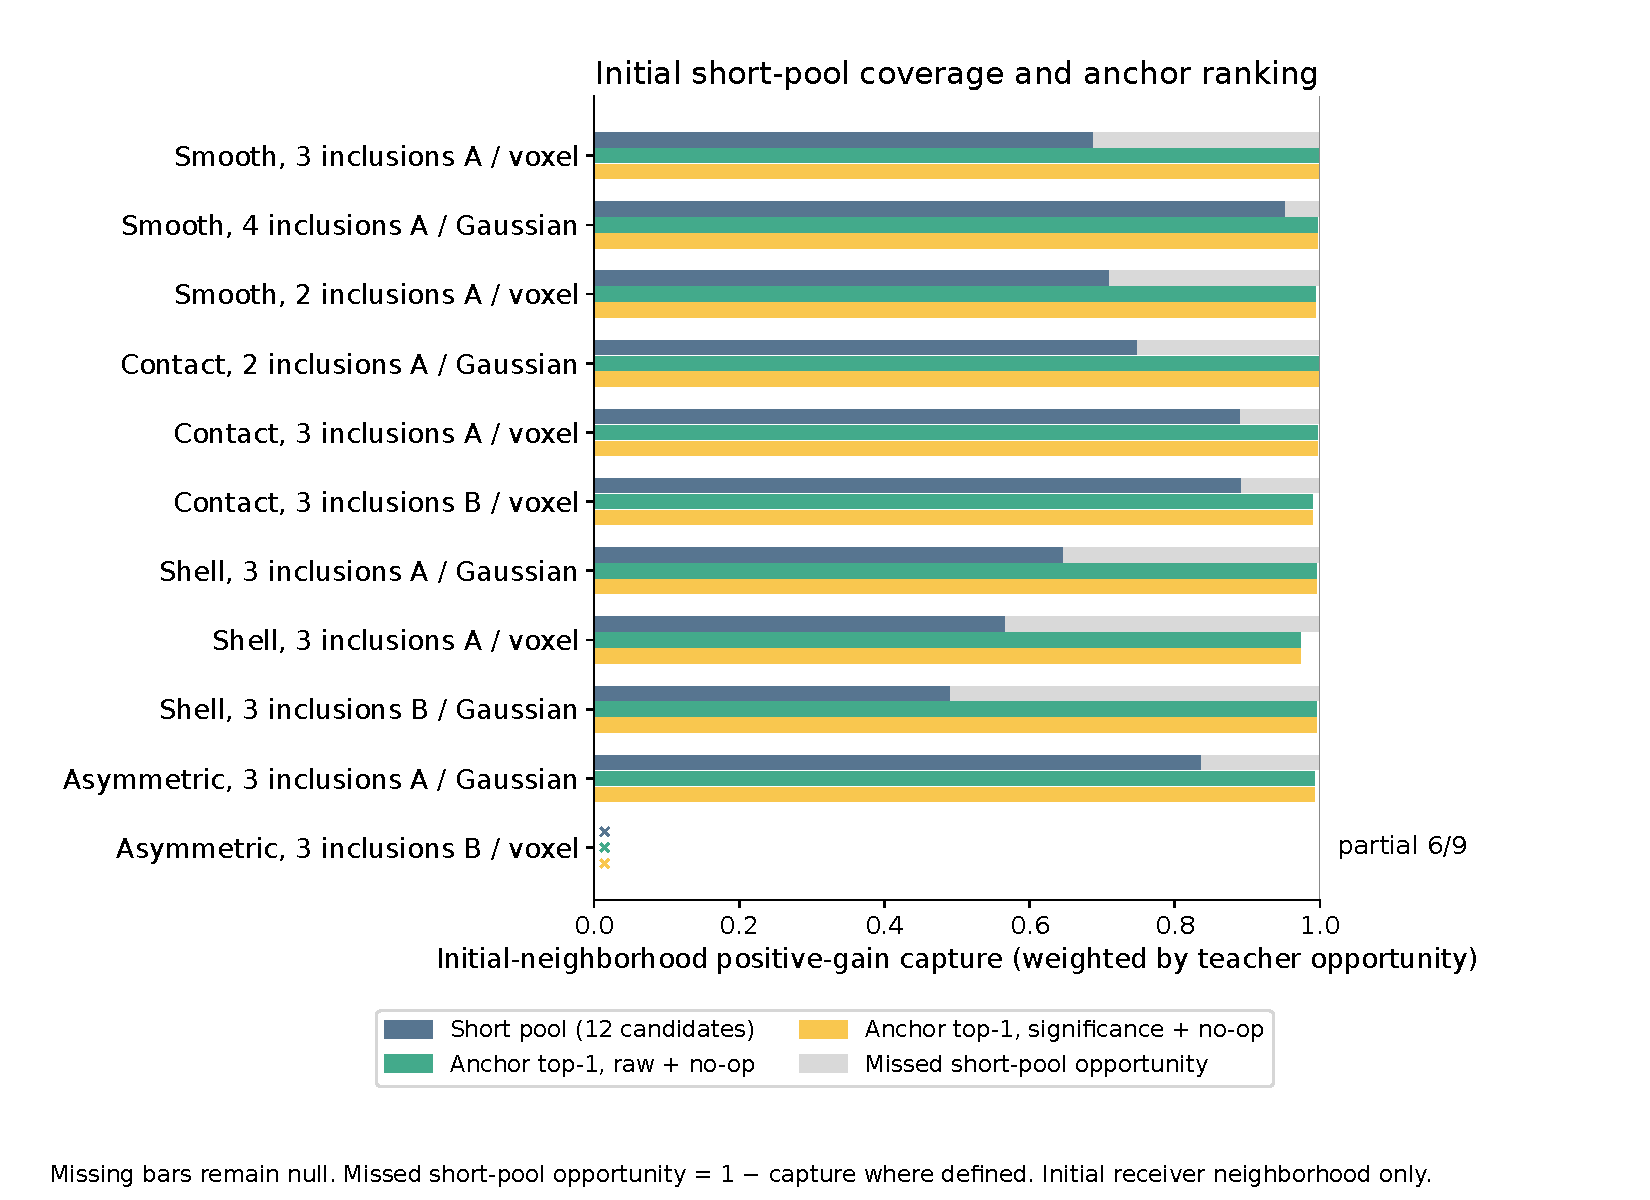
\includegraphics[width=.95\linewidth]{figures/coverage_closure_v2/initial_opportunity.pdf}
\caption{完整字典排序与固定短池覆盖是两个问题。图以对象内正收益求和后的比例呈现，非对称voxel对象的6/9观察结果单独标注。它不是最终重建误差，也不是部署整条路径的收益比例。}
\end{figure}

进一步的离线诊断最多走三个完整收益贪心动作，每次重新枚举当前邻域。它在90个单元得到更低终态gap；线上路径在5个单元更低；1个在评价底噪内相同。即使每一步都看整个字典，局部贪心也不保证全局最好，所以不能把所有终态差距称为“评分误差”。这里应分开三个问题：方向有没有送进来、送来的方向有没有排对、接受以后进入了哪个新邻域。改善候选取得是后续方向，当前冻结规则没有新增网络或再调短池。


\subsection{真正重建：为什么必须再检验一次}
冻结状态的GN比较把当前材料、总场和残差暂时固定。真正的非线性反演（nonlinear reconstruction）执行一步以后，这些量都会改变。还必须满足材料可行域（material feasibility constraints），并用线搜索（line search）判断新材料是否使完整非线性目标下降。因此，局部GN gap和最终材料误差（final material error）是两个不同指标。

固定的四个代表对象使用$k=8$，两种策略共享初始化$0.1+0.04i$、prior、LM schedule、实部下界$-0.5$、虚部下界0以及Armijo充分下降检验（Armijo acceptance）。每次先投影可行材料步，再从$\alpha=1$开始减半，最多24次；两条轨迹只改变切向电流空间。三组对照完成18次更新。

\begin{table}[htbp]\centering\small
\caption{完整三维材料相对误差：receiver $\to$ exchange。不是中心切片误差。}
\begin{tabular}{lrrr}\toprule
几何 / 表示&复材料&实部&虚部\\\midrule
平滑 / voxel&$0.3027\to0.2699$&$0.2811\to0.2516$&$0.7439\to0.6506$\\
近接触 / Gaussian&$0.6722\to0.6707$&$0.6810\to0.6835$&$0.4439\to0.2859$\\
shell / Gaussian&$0.6096\to0.5660$&$0.6081\to0.5651$&$0.6976\to0.6219$\\\bottomrule
\end{tabular}
\end{table}

三组复材料误差下降约10.8\%、0.22\%、7.16\%，留出测量误差（held-out data error）也下降。近接触对象尤其说明，数据拟合改善并不自动意味着材料所有分量改善：它的实部误差略升，复误差几乎中性。非对称voxel对象的exchange轨迹完成17次接受更新以后，在第18次更新前构建的receiver初始端点未通过预定法方程残差检查，故exchange轨迹停止。独立的receiver-only基线未运行；没有把最后安全状态当作完成终点，也不能据此推断未运行基线一定失败。

完整耗时（all-in wall time）包括每条轨迹自己的物理setup、anchor/pool获取、被拒绝的检查、line search和终点评价。三组耗时比是2.68、1.74、1.46；额外完整切向RHS分别为708、744、744，其中包含$Jx$初始化和$Jd$复核。这个方法的意义是用额外物理作用购买局部更新保真度，现有结果没有证明加速成像。

\begin{figure}[htbp]\centering
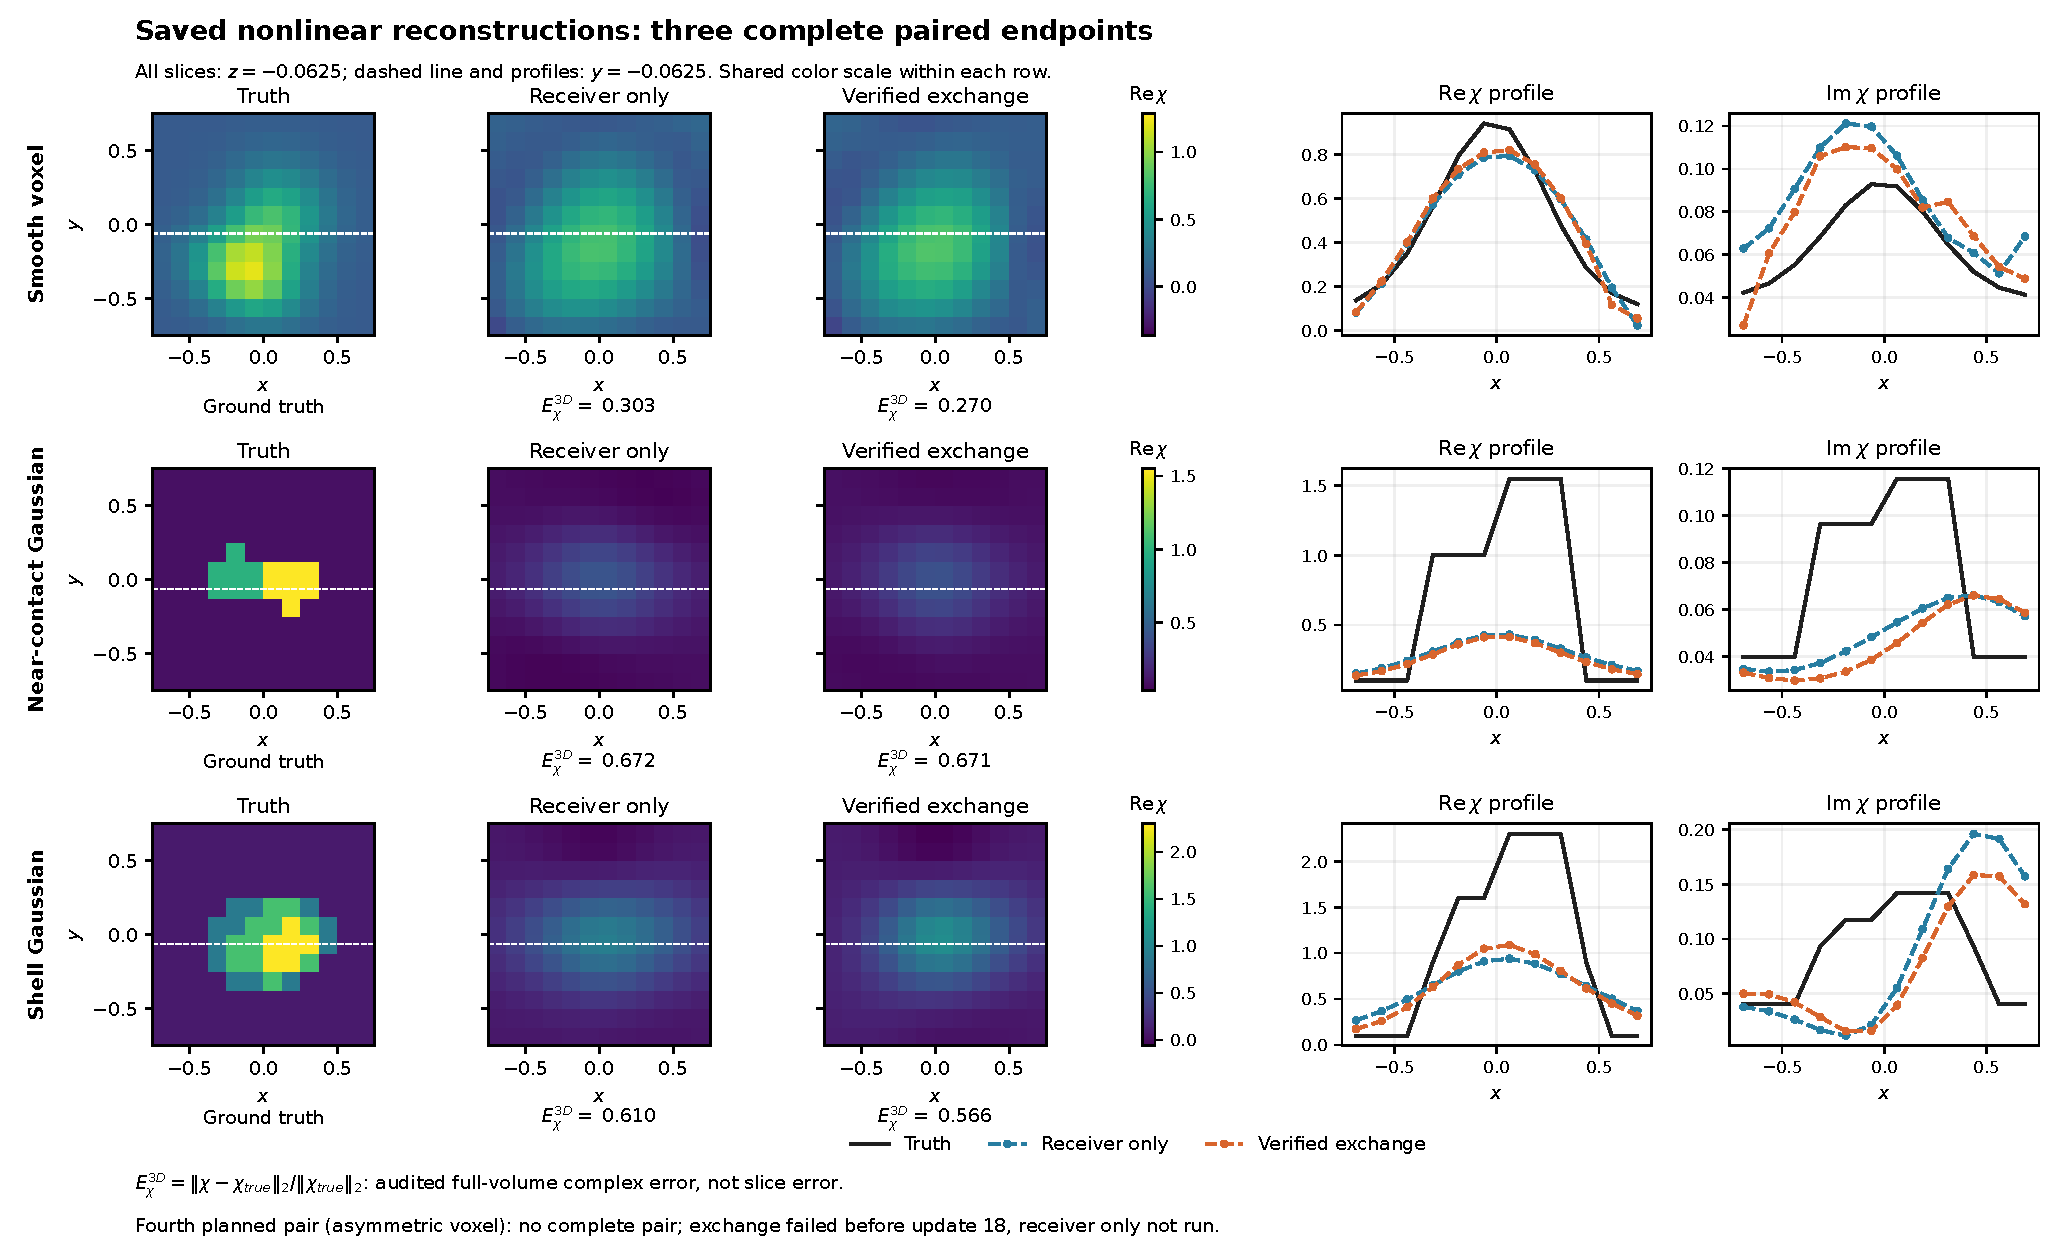
\includegraphics[width=.97\linewidth]{figures/nonlinear_closure_v1/nonlinear_reconstructions.pdf}
\caption{从左到右先看真实材料、receiver与exchange的同一中心切片，再看实部和虚部剖面线。每行统一色标，避免颜色范围不同制造视觉优势。整个体积上的误差见上表；切片仅帮助理解改善出现在哪里。接触与shell峰值仍被平滑，说明有限测量和材料表示仍限制恢复。}
\end{figure}

\begin{figure}[htbp]\centering
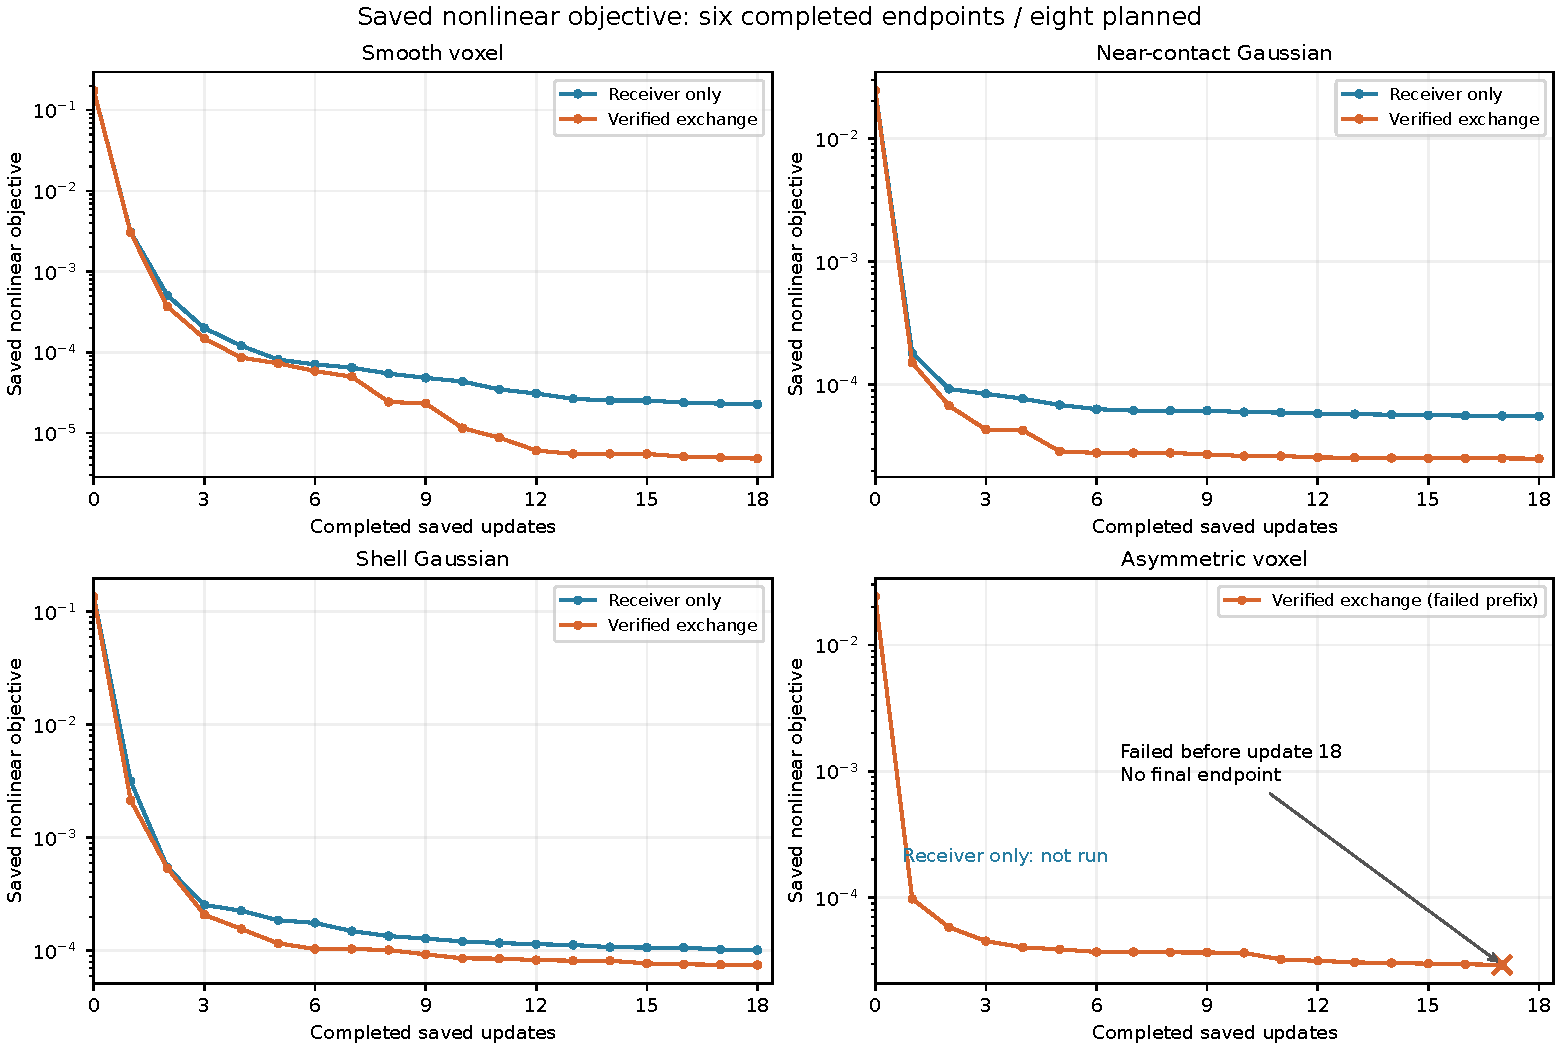
\includegraphics[width=.95\linewidth]{figures/nonlinear_closure_v1/nonlinear_objective_curves.pdf}
\caption{完整非线性目标（full nonlinear objective）随实际接受更新的变化。三个完整对照达到共同的18次更新上限。右下图单独保留非对称voxel的17步安全前缀，其后发生端点残差失败；没有对应的完成基线，不能把该曲线当作第四组成功。}
\end{figure}


\subsection{怎样阅读费用，而不被一个很快的局部耗时误导}
固定电流维数（fixed current dimension）只规定最后端点有多少列电流。为了选择这几列，exchange额外取得64列anchor、154方向字典，并支付每轮的完整方向核验（directional verification）。这些辅助信息并没有变成端点的额外列，但都需要计算和内存。被拒的候选同样已花费物理作用。

费用账本只把互不重叠的区间相加：原历史费用4889.515秒、61个闭合作业的15072.343秒，以及未进入作业的0.202秒检查，共19962.060秒，即5.545小时。子阶段、GPU上传和矩阵标签都是其中的细目，不应再加一遍。这个总数是研究执行成本，不是每个读者复现一次选择都需要的时间。

真正独立初始化的三对重建则能直接比较：receiver到exchange分别为216.46到579.89秒、407.71到710.49秒、405.90到592.29秒。三个比值都大于1。壳体所需完整forward RHS减少，总时间仍增加，说明一个环节省工作不等于整条流程加速。当前方法的工程作用是用额外计算得到更好的局部材料步，不是免费提高成像质量。


